\documentclass{chi-ext}
% Please be sure that you have the dependencies (i.e., additional LaTeX packages) to compile this example.
% See http://personales.upv.es/luileito/chiext/

%% EXAMPLE BEGIN -- HOW TO OVERRIDE THE DEFAULT COPYRIGHT STRIP -- (July 22, 2013 - Paul Baumann)
% \copyrightinfo{Permission to make digital or hard copies of all or part of this work for personal or classroom use is granted without fee provided that copies are not made or distributed for profit or commercial advantage and that copies bear this notice and the full citation on the first page. Copyrights for components of this work owned by others than ACM must be honored. Abstracting with credit is permitted. To copy otherwise, or republish, to post on servers or to redistribute to lists, requires prior specific permission and/or a fee. Request permissions from permissions@acm.org. \\
% {\emph{CHI'14}}, April 26--May 1, 2014, Toronto, Canada. \\
% Copyright \copyright~2014 ACM ISBN/14/04...\$15.00. \\
% DOI string from ACM form confirmation}
%% EXAMPLE END -- HOW TO OVERRIDE THE DEFAULT COPYRIGHT STRIP -- (July
%% 22, 2013 - Paul Baumann)

\title{Preserving Musical Performance on Touch-Screens}

\numberofauthors{4}
% Notice how author names are alternately typesetted to appear ordered in 2-column format;
% i.e., the first 4 autors on the first column and the other 4 auhors on the second column.
% Actually, it's up to you to strictly adhere to this author notation.
\author{
  \alignauthor{\hfill}\alignauthor{
    \textbf{Charles Martin}\\
    \affaddr{Research School of Computer Science, CECS}\\
    \affaddr{Australian National University, Canberra, ACT, 0200,
    Australia}\\
    \email{charles.martin@anu.edu.au}
  }
  \vfil
  \alignauthor{
    \hfill
  }\alignauthor{
    \textbf{Henry Gardner}\\
    \affaddr{Research School of Computer Science, CECS}\\
    \affaddr{Australian National University, Canberra, ACT, 0200,
    Australia}\\
  \email{henry.gardner@anu.edu.au}
  }
}

% Paper metadata (use plain text, for PDF inclusion and later re-using, if desired)
\def\plaintitle{CHI LaTeX Extended Abstracts Template}
\def\plainauthor{Luis A. Leiva}
\def\plainkeywords{Guides, instructions, author's kit, conference publications}
\def\plaingeneralterms{Documentation, Standardization}

\hypersetup{
  % Your metadata go here
  pdftitle={\plaintitle},
  pdfauthor={\plainauthor},  
  pdfkeywords={\plainkeywords},
  pdfsubject={\plaingeneralterms},
  % Quick access to color overriding:
  %citecolor=black,
  %linkcolor=black,
  %menucolor=black,
  %urlcolor=black,
}

\usepackage{graphicx}   % for EPS use the graphics package instead
\usepackage{balance}    % useful for balancing the last columns
\usepackage{bibspacing} % save vertical space in references

\usepackage{footmisc}


\begin{document}

\marginpar{\vspace{0.55cm}}

\marginpar{
\begin{figure}
\centering
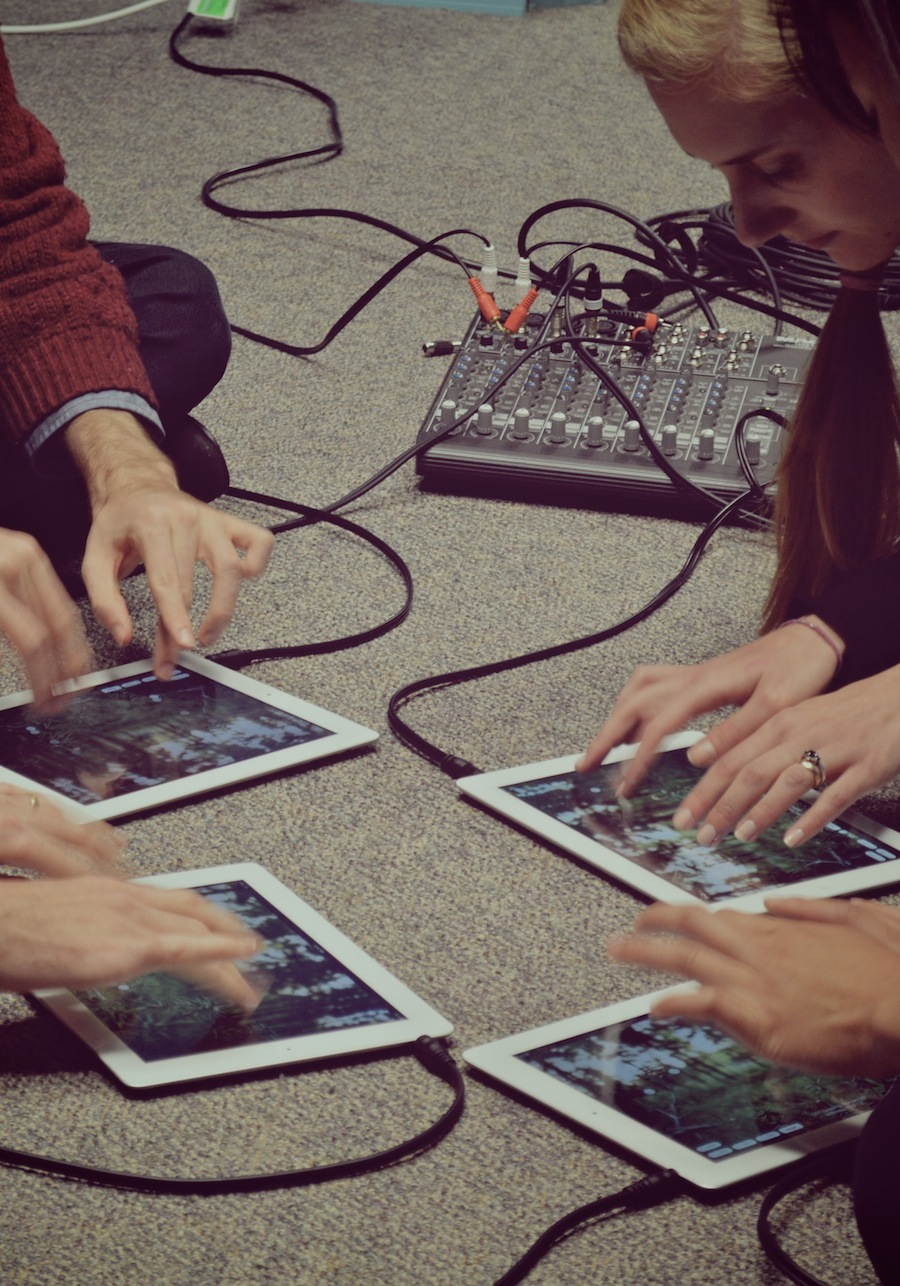
\includegraphics[width=0.8\columnwidth]{metatone-hands-long}
\caption{Ensemble Metatone performing with iPads and percussion instruments.}
\label{fig:EnsembleMetatone}
\end{figure}
}


\maketitle

\begin{abstract}
Musical performances with touch-screen devices can be recorded by
capturing a log of touch interactions. This new-media object can serve
as an archive or as a basis for other representations of the
musical work. This paper presents a protocol for logging
touch-interactions as well as visualisations and gesture-scores
generated from logs of a series of improvised ensemble performances on iPads. These objects record
the performances for posterity and also allow deeper analysis of
musical interactions present.
\end{abstract}

\keywords{improvisation, touch-screen, mobile music, visualisation,
  machine learning, gesture, archiving}

\category{H.5.5}{Sound and Music Computing}{Methodologies and techniques}.  


\section{Introduction}

When performing with touch-screen devices, musicians have the
opportunity to record the musical work in an extremely detailed
form by capturing a log of touch interactions with the devices. In
this paper, we argue that this log can form a new media object in
its own right, to be used as an archival
format and a basis for other representations of the work such as
visualisations or scores. We will describe the protocol for capturing
touch interactions with iPads developed for Ensemble Metatone, a
free-improvisation percussion group. Although this protocol was
developed for research purposes, visualisations and analyses generated
from logged data has formed an important archive of the group's
performances of \emph{MetaLonsdale} for four
iPads\footnote{\label{note1}The video recording,
  touch-interaction log, visualisation and score of a performance of
  \emph{MetaLonsdale} is available online: 
\url{http://charlesmartin.com.au/blog/2014/1/17/metalonsdale-for-four-ipads}.}

\subsection{Representing the Musical Work}

\marginpar{
\begin{figure}
  \centering
  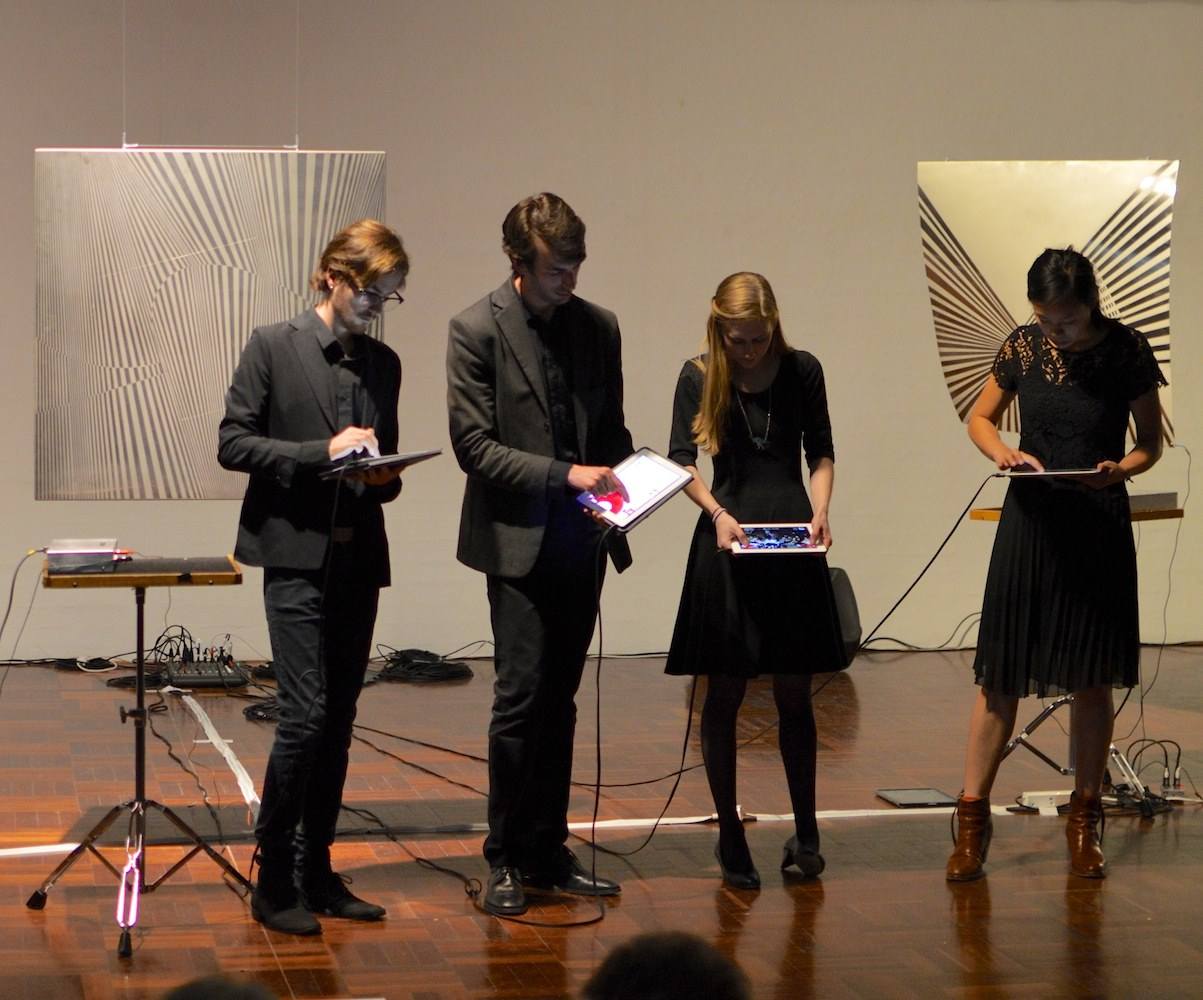
\includegraphics[width=\marginparwidth]{ensemblemetatone}
  \caption{Ensemble Metatone performing \emph{MetaLonsdale} at the ANU School of Art
    Gallery in October 2013 (left to right: Jonathan Griffiths,
    Charles Martin, Christina Hopgood, Yvonne Lam).}
  \label{ensemblemetatoneperforming}
\end{figure}
}

It is widely recognised that musical works as well as new media artefacts can have a number of
interacting representations~\cite{Rinehart:2007pi}. Musical works
might be directed by a score; be ``thick'' or ``thin''
depending on the the freedom of interpretation afforded the
performers; be represented in live performance, studio recordings, or
by computer generated renderings; and may be composed or improvised~\cite{Davies:2005fj}.
Combinations of these representations are often collected together
form an archive of a musical work.

Free improvised music, where performers do not follow a set musical
structure, is usually preserved using only audio and video recordings.
While the improvised solos of famous jazz musicians are often
transcribed, this is extremely uncommon
for free-improvised ensemble performances. For improvised music on
touch-screens, a log of 
touch-interactions captured by the performance suplements traditional
recordings and could take the place of a ``score'' in documenting
such performances. While scores are generally used for composition,
their use as documentation for new media artworks has been
acknowledged~\cite{MacDonald:2009ve}. Such a log would also satisfy Manovich's principles
for a new media artwork~\cite{Manovich:2002ly}. In particular, the log of
touch-interactions is variable, forming the basis for derivative
artworks that also represent aspects of the original performance. 

Free-improvisation is often a process of gestural exploration, discovering
new sounds and responding to other sounds in an ensemble. In audio
recordings of these performances, the sonic result of the gesture is
captured but the gesture itself lost. 
While the gestural component of musical
performance may not be as integral as in dance or other physical
performance, it still contributes to the audience's perception of a
work and represents a certain amount of the performers' intention.
Although touch-interaction data is not a complete record of
performers' gestures it is simple to obtain and easily transformed
into other representations of a performance.

\section{Ensemble Metatone and MetaLonsdale}

Ensemble Metatone was brought together to study the process of
performing free-improvised music on specially designed iPad apps and
percussion instruments in Canberra, Australia. The members of the group (including
one of the authors of this paper) are all trained in classical
percussion with experience as improvisors.

Over a series of studio rehearsals, the group worked with the
``MetaLonsdale'' app to develop a work which was performed at
festivals and events throughout 2013. The studio rehearsals and a public recital were
recorded with seperate tracks of audio for each iPad, multiple camera angles, and a log of touch-interactions.

The app used a percussion-inspired interaction scheme allowing
performers to access pitched percussion sounds and field recordings.
Most of the iPad screen was a performance surface with few graphical
UI elements. Tapping the screen produced short sounds at a pitch
determined by the location of the tap. Swiping played continuous field
recordings with volume controlled by the velocity of the swipe. The
app featured two UI switches that controlled simple delay functions, that repeat tapped notes, and
switchable auto-play features, that alogrithmically produced
background sounds. A button on both apps allowed the performer to shuffle
the available sounds.

\marginpar{
\begin{figure}
  \centering
  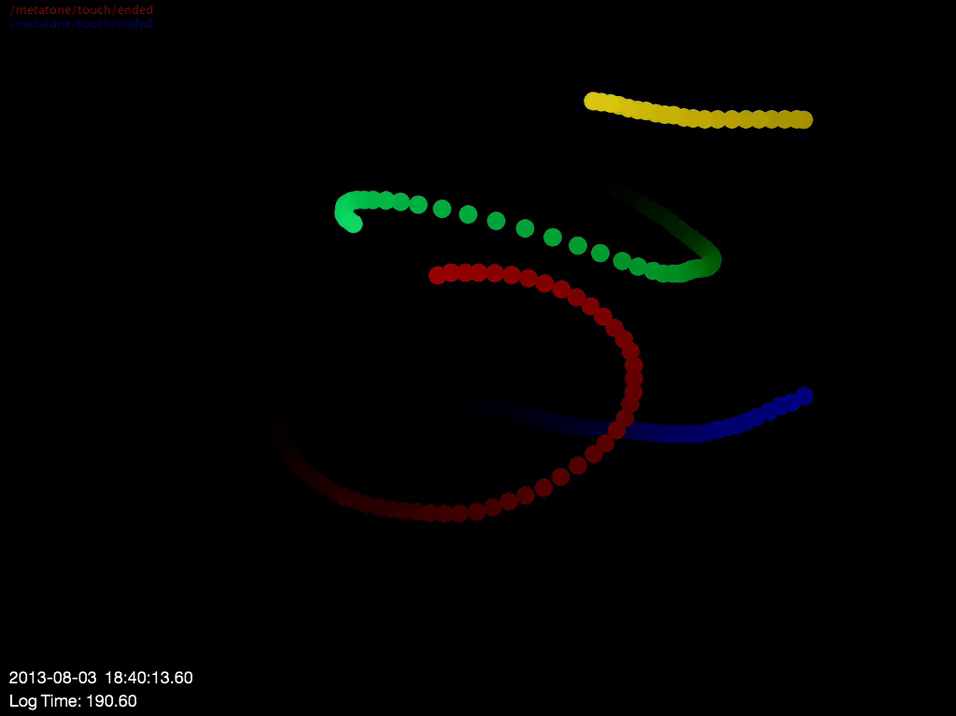
\includegraphics[width=\marginparwidth]{metatoneanimation1}
  \label{metatoneanimation1}
\end{figure}
\begin{figure}
  \centering
  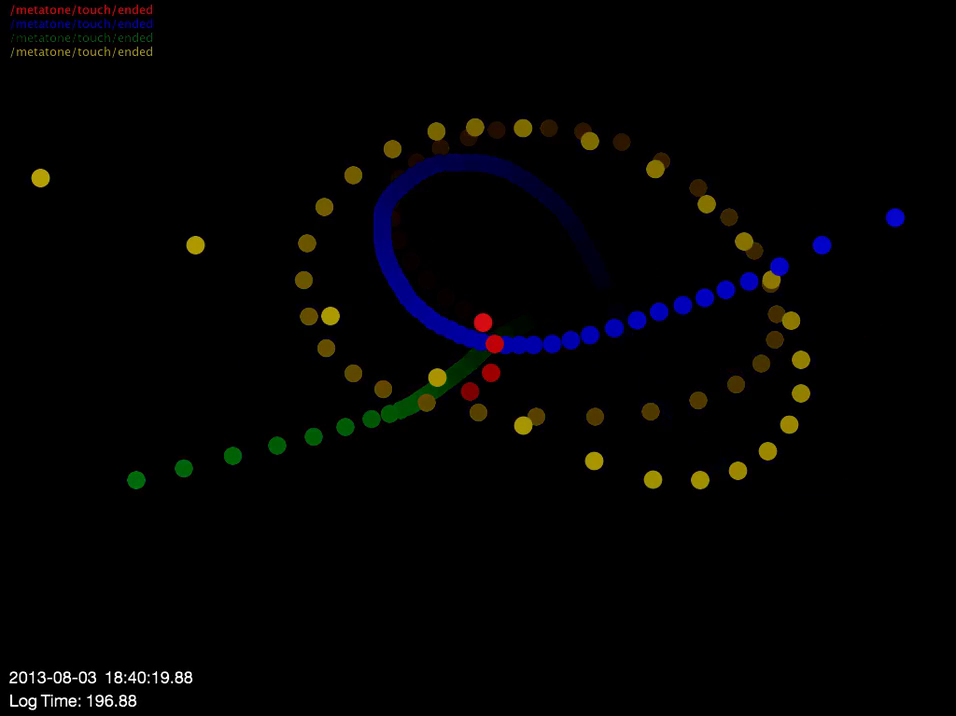
\includegraphics[width=\marginparwidth]{metatoneanimation3}
  \label{metatoneanimation2}
\end{figure}
\begin{figure}
  \centering
  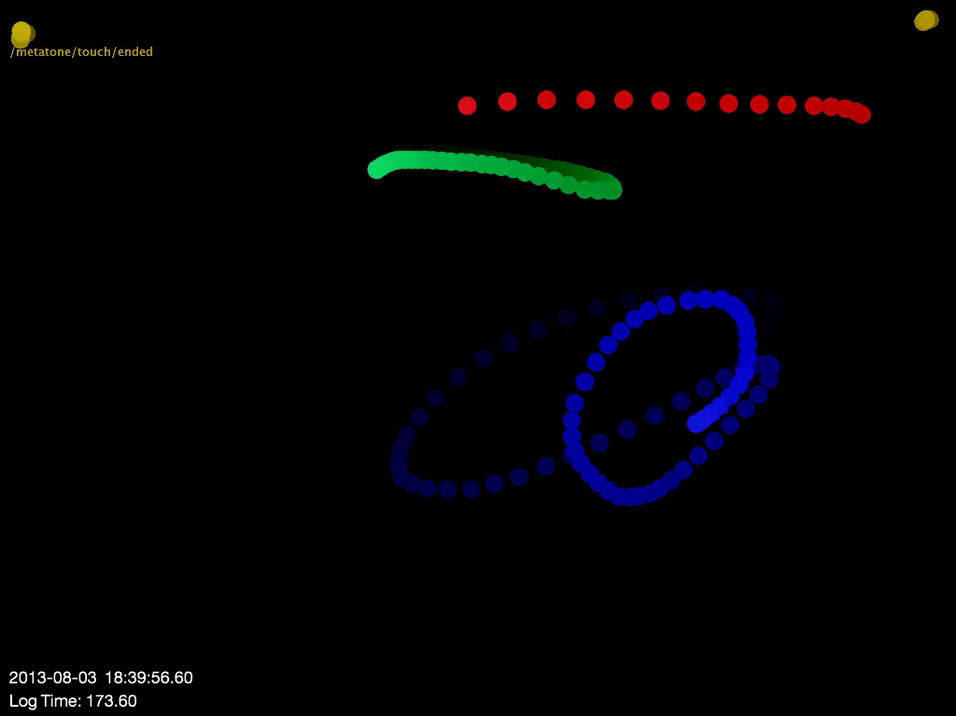
\includegraphics[width=\marginparwidth]{metatoneanimation2}
   \caption{Stills from an animation of an Ensemble Metatone
     performance. The full animation can be viewed online\footref{note1}.}
  \label{metatoneanimation3}
\end{figure}}

\section{Capturing Data}

Touch interactions were transmitted as OSC
messages over a Wi-Fi network from the four iPads to a laptop. 
Messages from touches in the performance area
were sent with the location of the touch and velocity. Touch-down
events were denoted with a velocity of zero while touch-ended events
were represented with a different OSC address. Messages were also sent
when the button was pressed or a switch was moved in the UI. A logging application
on the laptop assigned timestamps to each message and wrote
it to a text file for later analysis. 

This scheme for logging touch-interactions (see table \ref{oscschema}) was chosen to study the
process of improvising with iPad instruments and not necessarily for
replaying performances. It does not capture other touch ``state'' variables
such as a unique identifier for each touch. It also does not attempt
to keep track of OSC messages that might be delayed or lost, or
network communications that took place between the iPads.
However, the log is extremely useful as a recording of interaction
with the instruments and can be transformed into other representations
of the performance. While the logs were created for research purposes
they also serve as representative artefacts of the performance along
with the audio and video recordings.

\begin{table}
  \begin{tabular}{|l|l|}
  \hline
  OSC Address           & Parameters \\ \hline
  /metatone/online      & device  \\     
  /metatone/touch       & device, X, Y, velocity \\
  /metatone/touch/ended & device \\  
  /metatone/switch      & device, switch, position\\ \hline
  \end{tabular}
  \caption{Scheme for OSC messages from the Metatone iPad apps. The
    switch message was also used to record presses of the UI button in
    the app.}
  \label{oscschema} 
\end{table}

\subsection{Animations}

To understand the structure of the improvised performances we wanted a
visual representation of the performers' touch gestures to watch
alongside the audio and video recordings of each performance. A
Processing sketch was produced that read the captured log files and
rendered an animation of all four players' touches in the space of one
iPad screen with different players distinguished by colour. The sketch
also draws a date and time stamp on each frame as well as text
notifications of switch and button messages.

The resulting animations presents an entirely new view of the
performance which was not visible to the performers or audience on the
day.
As all the touch movements are layered in one performance area it is
immediately clear when performers mimic each other, form sections, or
experiment with a new musical idea. From the
researcher's point of view, the animation also gives a ``performer's
perspective'' on touch interaction, allowing us to connect patterns of
touches with musical gestures that the performers discuss after
rehearsals.

%\marginpar{\vspace{-10cm}}

\subsection{Tracking Gestures as a Score}

Interpreting the gestures of musicians improvising on touch-screen
instruments was a research goal of working with Ensemble Metatone. One
approach to this has been the application of machine-learning
algorithms to logs of touch-interaction. After the initial rehearsal
series took place, a vocabulary of touch gestures was developed from
qualitative analysis of the rehearsals and discussions among the
performers. From this vocabulary, examples of each gesture were
recorded and the resulting log used to train a Random Forest
Classifier algorithm~\cite{Breiman:2001kx}. Five second windows in the logs are used to calculate
feature vectors which are classified by the algorithm. While research
into how this technique can be applied in live performance is ongoing,
the classifier is able to produce an interpretation of recorded
performances as a ``score'' of gestures. In figure \ref{gesturescore},
each performer's gesture is given by the coloured lines which can move
between the nine possible gestures in the vocabulary. Graphical scores
like figure \ref{gesturescore} are common in contemporary music and
the representation of a performance as a sequence of gestures recalls
descriptions of free-improvised music as ``transitions'' and
``attractors''~\cite{Stenstrom:2009xy}. 

\marginpar{
\begin{figure}
\centering
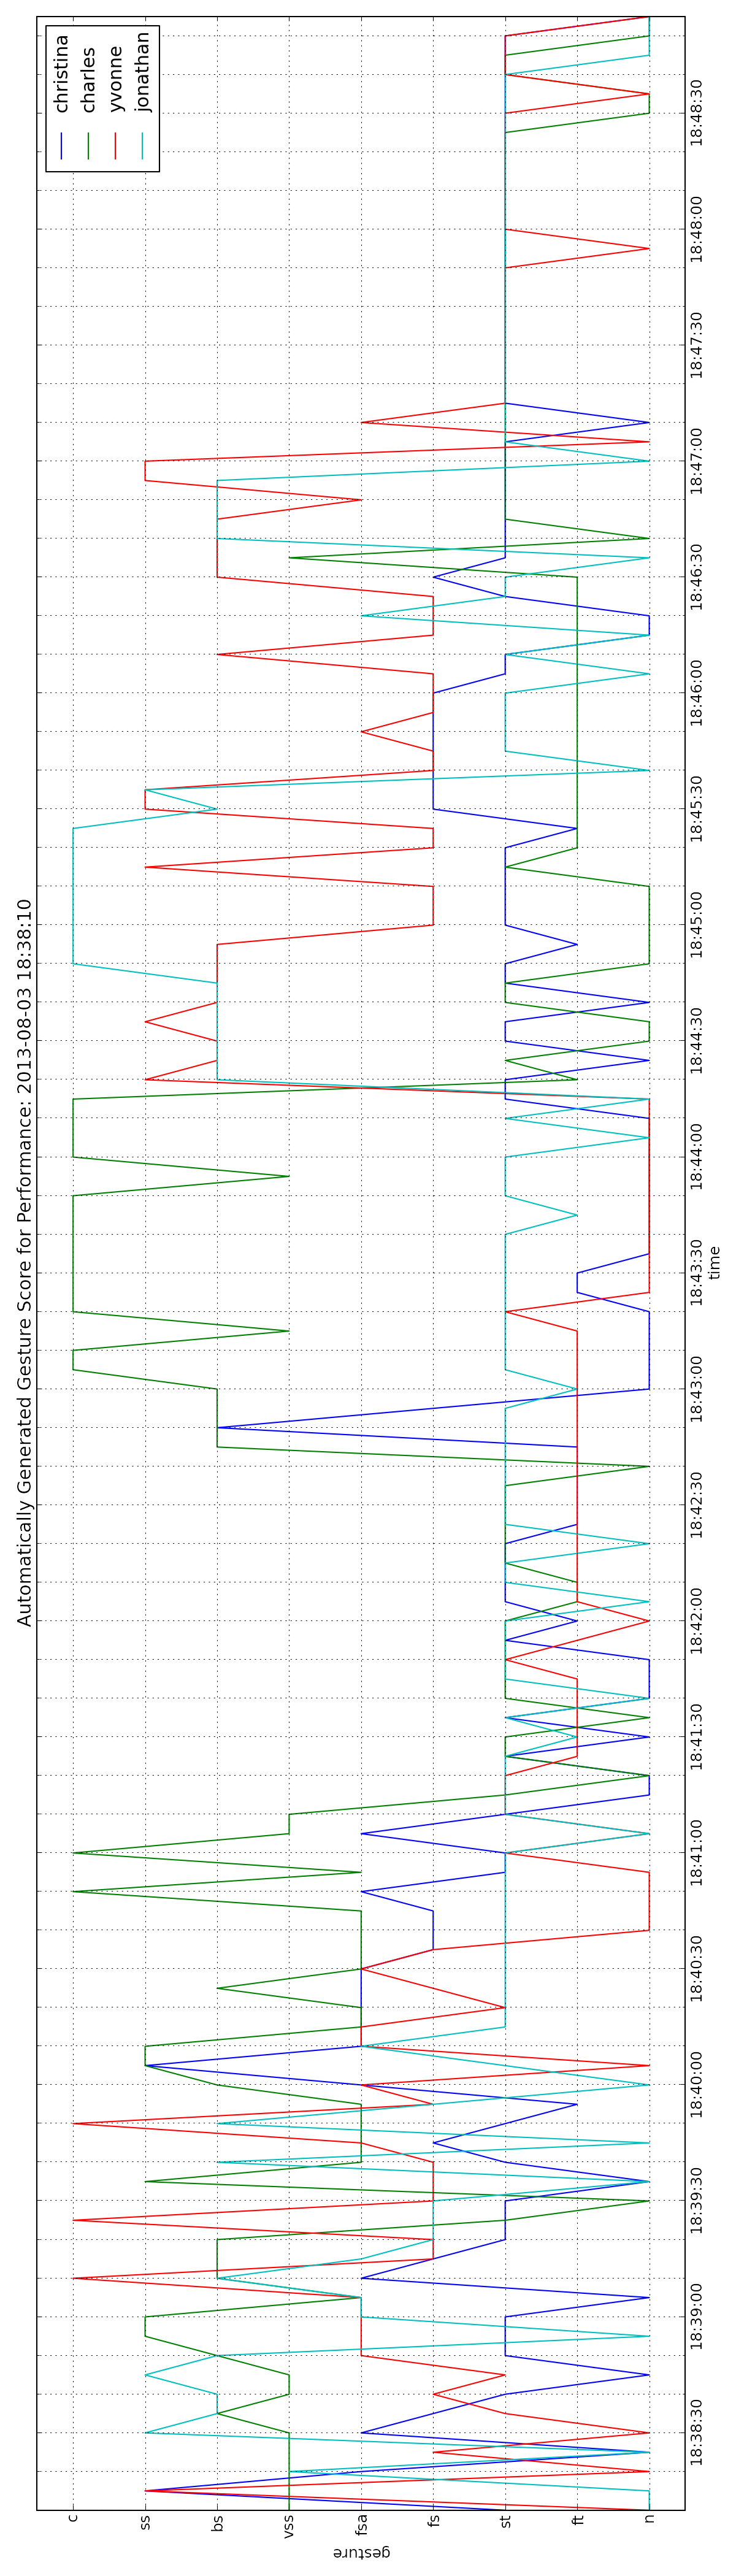
\includegraphics[width=0.9\marginparwidth]{score20130803vert}
\caption{An automatically generated ``gesture score'' for the
  \emph{MetaLonsdale} performance on 3-8-2013. }
\label{gesturescore}
\end{figure}}

The scores produced so far are already helpful in understanding at a
glance the overall flow of a performance. In this way they may be more
useful archival documents of a performance than, for example, a still
photograph of the stage setup.

\section{Conclusions}

By logging touch-interactions in Ensemble Metatone's performances on
iPads we recorded aspects of the musical work that are not accessible
in traditional archives of free-improvised music. The logs also allow
further insight into the gestural nature of performance on
touch-screens. In particular, animations of the performers' touches
aided the development of a vocabulary of gestures.  Graphical
``gesture scores'' following this vocabulary were generated from
the logs automatically using a Machine-Learning algorithm. 

These alternative representations have allowed a more comprehensive archive
of performances and one that affords more insight into the performers'
gestural and musical intent and ensemble interactions as well as
their sonic output. As more performances are logged, it is hoped that
these representations will allow us to track the group's musical
developments or different approaches taken with future touch
instruments. The representations could also be used in performance as
visual accompaniments for the audience or displayed to the players as
real-time feedback.

\balance
\bibliographystyle{acm-sigchi}
\bibliography{2013ComputerMusic}

\end{document}